\section{Moduł ECG\_BASELINE}

\subsection{Wstęp}

Zagadnienie usuwania zakłóceń z sygnału EKG jest szeroko omawiane w literaturze. Wynika to z popularności badania, a także wyzwania stawianego inżynierom -- sygnał ten ma niewielką amplitudę, a zakłócenia pochodzą z wielu źródeł -- głównie mięśni, elektrod, linii zasilającej urządzenia badawczego i rytmu oddechowego pacjenta \cite{Sayadi2008}.  Kolejnym utrudnieniem jest fakt, że ich pasmo zakłóceń zazwyczaj pokrywa się z sygnałem użytecznym -- zachodzi więc obawa, że wstępne filtrowanie sygnału może zniekształcić jego interesującą część \cite{Jane1992}. 

W ciągu ostatnich dekad wielu naukowców pracowało nad opracowaniem metod usuwania szumu z sygnału EKG. Manpreet Kaur \cite{Kaur2011} w swym przeglądzie porównuje filtry IIR, FIR, średnią kroczącą, metodę splajnów oraz oparty o transformację falkową. Ten ostatni dekomponuje sygnał w bazie db4, a następnie usuwa tę część sygnału, która jest najwolniej zmienna. Filtrem najlepiej odszumiającym sygnał okazał się IIR o zerowym przesunięciu fazowym. Jego wyjście cechowało się najwyższym SNR oraz brakiem modyfikacji sygnału użytecznego. Na chwilę obecną prawdziwe wyzwanie stanowi jednak filtrowanie EKG płodu. Jego odczyt przy szumie pochodzącym od EKG matki jest wyjątkowo trudny \cite{Prasanth2013}. Nastała potrzeba opracowania skuteczniejszych metod filtracji sygnału.

W ostatnich latach popularność zyskała metoda filtracji sygnału w oparciu o adaptacyjny filtr Kalmana, ze względu na jego zdolność do jednoczesnego modelowania zarówno sygnału EKG, jak i izolinii \cite{Sayadi2008,Mneimneh2006}.  Naukowcy z Marquette University w swym artykule \cite{Mneimneh2006} wykazali wyższą skuteczność w usunięciu izolinii dla filtru Kalmana, zbudowanego w oparciu o model autoregresyjny, w porównaniu do średniej kroczącej i metody splajnów rzędu trzeciego. Charakteryzował się on nie tylko mniejszą średnią wariancją błędu, lecz także mniejszym zniekształceniem sygnału użytecznego w porównaniu do pozostałych. Niestety, zastosowane podejście okazało się nieskuteczne w przypadku szybkich zmian poziomu izolinii. Przyjęcie liniowego modelu EKG wydaje się zbytnim uproszczeniem.

Alternatywne podejście, wykorzystujące rozszerzony filtr Kalmana, zostało zaprezentowane w \cite{Sameni2005-1, Sameni2005-2}. Jego genezę stanowiły prace nad stworzeniem generatora EKG, opartego na nielinowym modelu matematycznym, uwzględniającym morfologię kompleksu QPRST i kształtu fali R-R. Jego prostota i elastyczność umożliwiają dobrą estymację sygnału EKG, również w przypadku jego chwilowego zaniku. W ramach swych prac autorzy udostępnili również narzędzie do automatycznej optymalizacji parametrów modelu. Naszym zdaniem wykorzystanie rozszerzonego filtru Kalmana, w oparciu o wyżej wspomniany model, to najbardziej obiecujący sposób na usunięcie szumu z zapisu EKG. Z uwagi na pracę off-line, kwestie złożoności obliczeniowej takiego rozwiązania są mniej ważne od jego ostatecznej skuteczności. 

W module ECG\_BASELINE zaimplementowane zostały następujące metody filtracji sygnału EKG: 
\begin{itemize}
\item Filtr Butterwortha (do usunięcia falowania izolinii oraz szumu sieci elektrycznej 50 Hz)
\item Średnia krocząca
\item Filtr Savitzky'ego-Golay'a
\item Rozszerzony filtr Kalmana
\end{itemize}

\subsection{Proponowane rozwiązanie}

W sekcji tej opisane zostały zaimplementowane filtry, z pominięciem filtru Savitzky'ego-Golay'a, ze względu na brak zmian w jego obrębie w stosunku do poprzedniej wersji modułu ECG\_BASELINE, opisanej w pracy~\cite{Baseline2013}.

\subsubsection{Filtr Butterwortha}

Filtr Butterwortha jest filtrem cyfrowym o nieskończonej odpowiedzi impulsowej (IIR -- \emph{Infinite Impulse Response}. Jest on odpowiednikiem filtru analogowego i ma realizowalną fizycznie transmitancję. W dowolnej chwili, wyjście filtru zależy od $N$ próbek wejściowych i $N$ poprzednich próbek wyjściowych, gdzie $N$ oznacza rząd filtru. Taka budowa prowadzi do problemów w implementacji -- ze względu na niezerowy błąd wynikający ze skończonej długości reprezentacji liczby zmiennoprzecinkowej, filtr IIR wysokiego rzędu będzie niestabilny numerycznie. W celu osiągnięcia odpowiedniej charakterystyki filtru, przy jednoczesnym uniknięciu problemów ze stabilnością numeryczną, filtry o nieskończonej odpowiedzi impulsowej implementuje się jako kaskadowo połączone sekcje filtrów drugiego rzędu. Transmitancja takiej sekcji wyraża się równaniem

\begin{equation}
H(z) = \frac{b_0 + b_1z^{-1} + b_2z^{-2}}{1 + a_1z^{-1} + a_2z^{-2}}
\end{equation}

Bezpośrednie wykorzystanie filtru Butterwortha napotykać może problemy wynikające z silnego, nieliniowego zniekształcenia fazy w okolicy częstotliwości odcięcia. Kolejnym problemem jest duże zniekształcenie sygnału w pierwszych sekundach przetwarzanego sygnału (\emph{transient}), mogące utrudnić działanie algorytmów automatycznej analizy sygnałów EKG. W celu rozwiązania tych problemów, stosuje się nieprzyczynowy filtr o zerowym przesunięciu fazowym, o strukturze przedstawionej na rysunku~\ref{fig:0phase} oraz rozszerza się sygnał o część przebiegu odbitą względem $OX$. Liczbę odbitych próbek oblicza się ze wzoru

\begin{equation}
t_r = \ceil{\min_k\frac{\pi}{\abs{p_k} \cdot \varphi(p_k)}}
\end{equation}

gdzie $p_k$ to bieguny transmitancji filtru, zaś $\varphi(p_k)$ określa argument zmiennej zespolonej $p_k$.

\begin{figure}[H]
\centering
	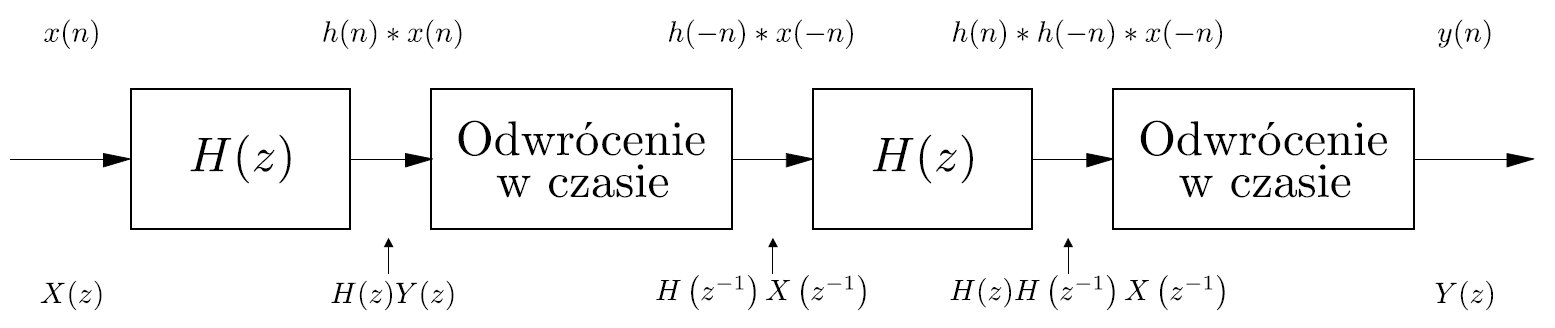
\includegraphics[width=\textwidth]{ECG_BASELINE/figures/butter_0phase.png}
\caption{Struktura nieprzyczynowego filtru o zerowym przesunięciu fazowym. Źródło: \cite{Baseline2013}}
\label{fig:0phase}
\end{figure}

Kolejnym problemem, na jaki natrafić można przy implementacji filtrów IIR jest ich niestabilność. Wszystkie filtry o skończonej odpowiedzi impulsowej (FIR -- \emph{Finite Impulse Response}) są z natury stabilne, ze względu na postać ich transmitancji -- brak w nich sprzężenia zwrotnego, przez co wszystkie ich bieguny znajdują się w początku układu współrzędnych. Filtry IIR posiadają sprzężenie zwrotne, przez co mogą być niestabilne -- w trakcie ich projektowania należy zadbać, aby wszystkie bieguny znajdowały się w obrębie okręgu jednostkowego na płaszczyźnie zespolonej $\mathbb{C}$. Wszystkie filtry opisane w tej pracy spełniają ten warunek.

Dla filtru Butterwortha dostępne w aplikacji są następujące zestawy współczynników:

\begin{itemize}

\item Usunięcie falowania izolinii
\begin{itemize}
\item Rząd filtru: 10 (rząd efektywny: 20)
\item Filtr wysokoprzepustowy, punkt -3db ustawiony na 0.5 Hz
\item Częstotliwości próbkowania: 250/360 Hz
\end{itemize}

\item Usunięcie szumu sieci elektrycznej 50 Hz
\begin{itemize}
\item Rząd filtru: 10 (rząd efektywny: 20)
\item Film pasmowozaporowy, punkty -3db ustawione na 49.5 Hz i 50.5 Hz
\item Częstotliwości próbkowania 250/360 Hz
\end{itemize}

\item Usunięcie 3 składowej harmonicznej szumu sieciowego o częstotliwości 150 Hz
\begin{itemize}
\item Rząd filtru: 10 (rząd efektywny: 20)
\item Filtr pasmowozaporowy, punkty -3db ustawione na 149.5 Hz i 150.5 Hz
\item Częstotliwość próbkowania: 360 Hz
\end{itemize}

\end{itemize}

Współczynniki oraz charakterystyki poszczególnych filtrów zostaną teraz przedstawione dla pojedynczej częstotliwości próbkowania.

\subsubsection{Filtr usuwający falowanie izolinii}

Współczynniki filtru dla częstotliwości próbkowania $f_s=250 Hz$ zebrane zostały w tabeli~\ref{tab:bw_250}. Charakterystyka amplitudowa i charakterystyka fazowa przedstawione zostały na rysunku~\ref{fig:bw_250}.

\begin{table}[H]
\begin{center}
\begin{tabular}{|c|c|c|c|c|}
\hline
        $b_0$ & $b_1$ & $b_2$ & $a_1$ & $a_2$ \\
\hline
        1& -2& 1& -1.99591858803741& 0.996076189822218\\
\hline
        1& -2& 1& -1.98849798039776& 0.988654996236322\\
\hline
        1& -2& 1& -1.98222892979253& 0.982385450614125\\
\hline
        1& -2& 1& -1.97769893355394& 0.977855096677832\\
\hline
        1& -2& 1& -1.97532566755629& 0.975481643282286\\
\hline
\end{tabular}
\caption{Współczynniki filtru Butterwortha do usuwania falowania izolinii dla $f_s=250 Hz$}
\label{tab:bw_250}
\end{center} 
\end{table}

\begin{figure}[H]
\centering
	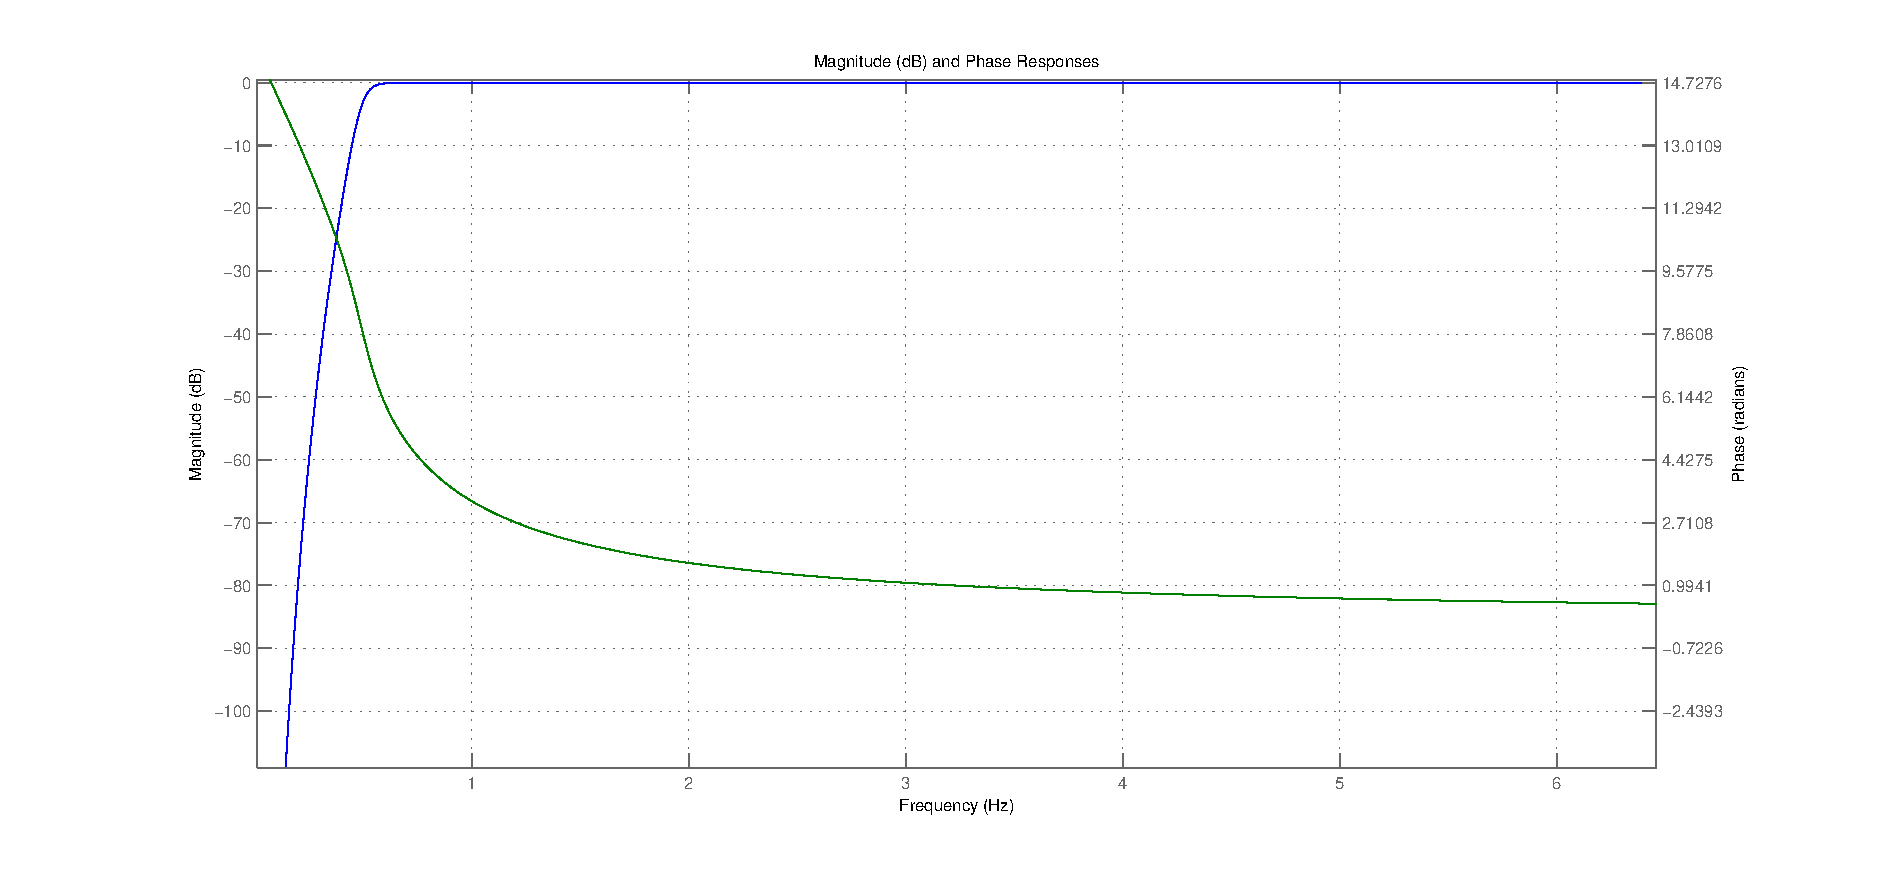
\includegraphics[width=\textwidth]{ECG_BASELINE/figures/bw_250.eps}
\caption{Charakterystyka amplitudowo i charakterystyka fazowa filtru Butterwortha do usuwania falowania izolinii dla $f_s=250 Hz$}
\label{fig:bw_250}
\end{figure}


\subsubsection{Filtr usuwający szum sieci elektrycznej 50 Hz oraz jego 3. harmoniczną}

Współczynniki filtru usuwającego szum sieciowy 50 Hz z sygnału próbkowanego z $f_s = 360$  zebrane zostały w tabeli~\ref{tab:ac_360}. Charakterystyka amplitudowa i charakterystyka fazowa przedstawione zostały na rysunku~\ref{fig:50hz_360}.

\begin{table}[H]
\begin{center}
\begin{tabular}{|c|c|c|c|c|}
\hline
        $b_0$ & $b_1$ & $b_2$ & $a_1$ & $a_2$ \\
\hline
        1& -1.28562417200218& 1& -1.26937327532045&        0.994584016960900\\
\hline
        1& -1.28562417200218& 1& -1.29478401747452&        0.994658733271036\\
\hline
        1& -1.28562417200218& 1& -1.26873553509657&        0.985919061981878\\
\hline
        1& -1.28562417200218& 1& -1.28442034996815&        0.986038923952812\\
\hline
        1& -1.28562417200218& 1& -1.27450176361204&        0.982697263115690\\
\hline
\end{tabular} 
\caption{Współczynniki filtru Butterwortha do usuwania szumu sieciowego 50 Hz dla $f_s=360 Hz$}
\label{tab:ac_360}
\end{center}
\end{table}

\begin{figure}[H]
\centering
	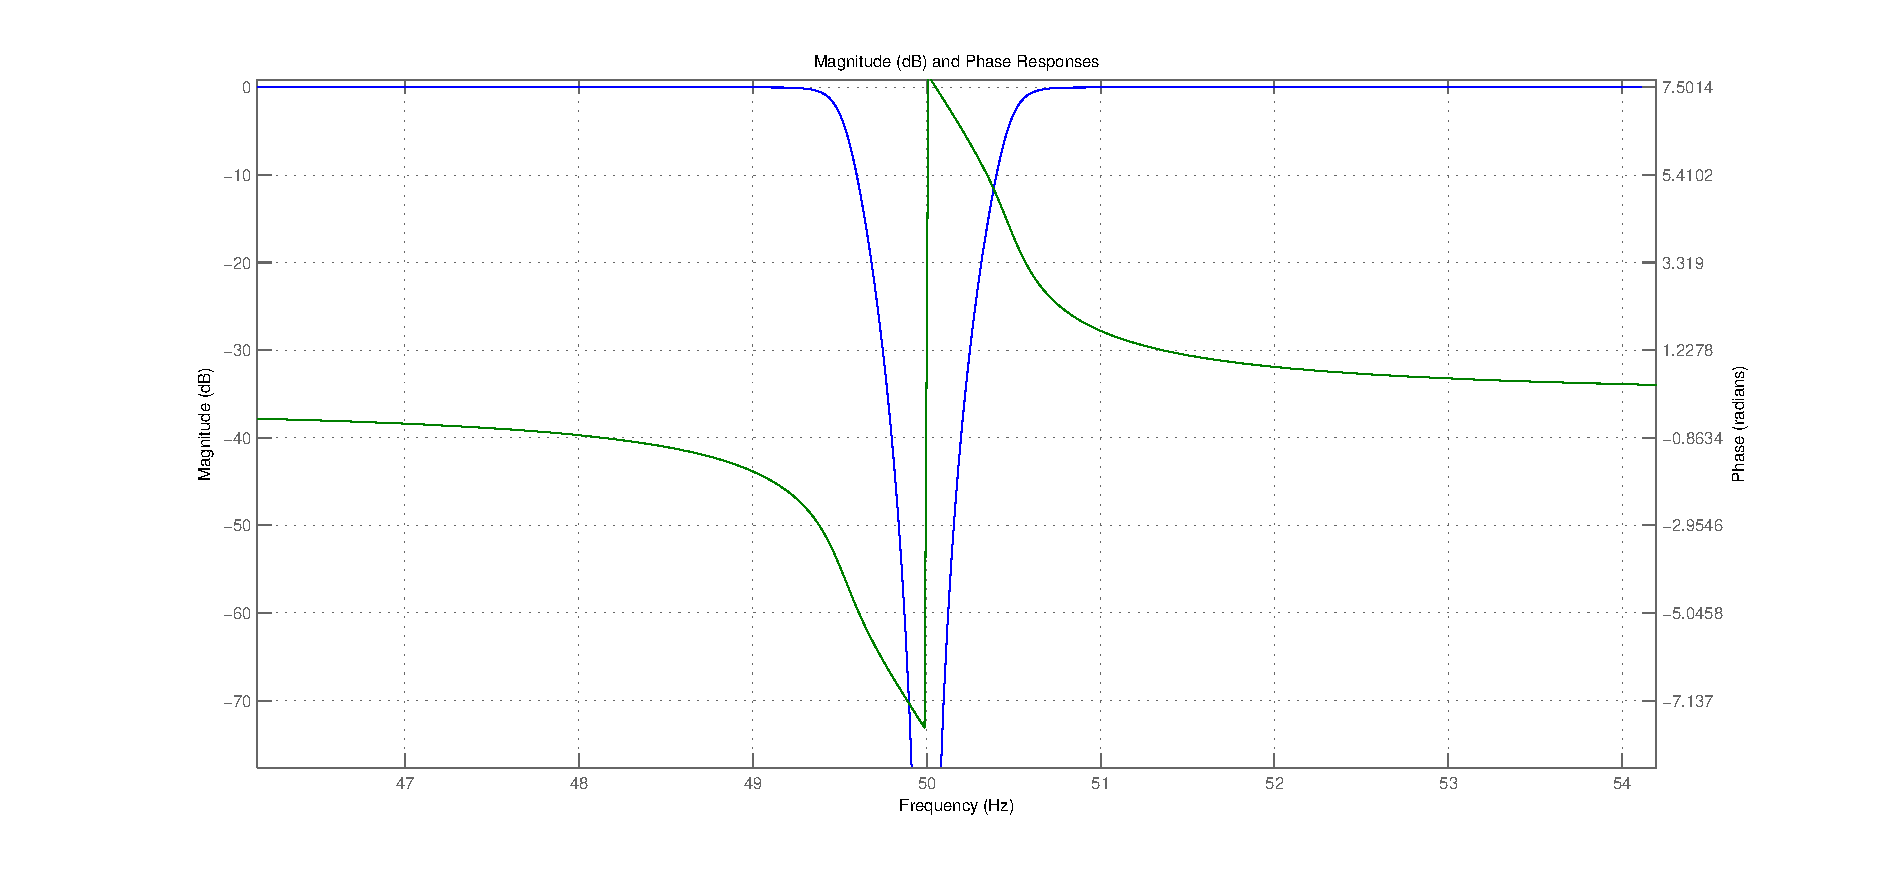
\includegraphics[width=\textwidth]{ECG_BASELINE/figures/50hz_360.eps}
\caption{Charakterystyka amplitudowa i fazowa filtru Butterwortha do usuwania szumu sieciowego 50 Hz dla $f_s=360 Hz$}
\label{fig:50hz_360}
\end{figure}

\newpage{}

Współczynniki filtru usuwającego 3. harmoniczną szumu sieciowego 50 Hz dla częstotliwości próbkowania sygnału $f_s = 360 Hz$ zebrane są w tabeli~\ref{tab:ac_3rd_360}. Charakterystyka amplitudowa i charakterystyka fazowa przedstawione zostały na rysunku~\ref{fig:3rd_360}.

\begin{table}[H]
\begin{center}
\begin{tabular}{|c|c|c|c|c|}
\hline
        $b_0$ & $b_1$ & $b_2$ & $a_1$ & $a_2$ \\
\hline
        1& 1.73211676126764& 1&        1.71899593699765& 0.994544262243386\\
\hline
        1& 1.73211676126764& 1&        1.73568383808774& 0.994698492564272\\
\hline
        1& 1.73211676126764& 1&        1.71472803758620& 0.985855276540036\\
\hline
        1& 1.73211676126764& 1&        1.72512958096071& 0.986102721276756\\
\hline
        1& 1.73211676126764& 1&        1.71713158098109& 0.982697263115690\\
\hline
\end{tabular} 
\caption{Współczynniki filtru Butterwortha do usuwania 3. harmonicznej szumu sieciowego 50 Hz dla $f_s=360 Hz$}
\label{tab:ac_3rd_360}
\end{center}
\end{table}

\begin{figure}[H]
\centering
	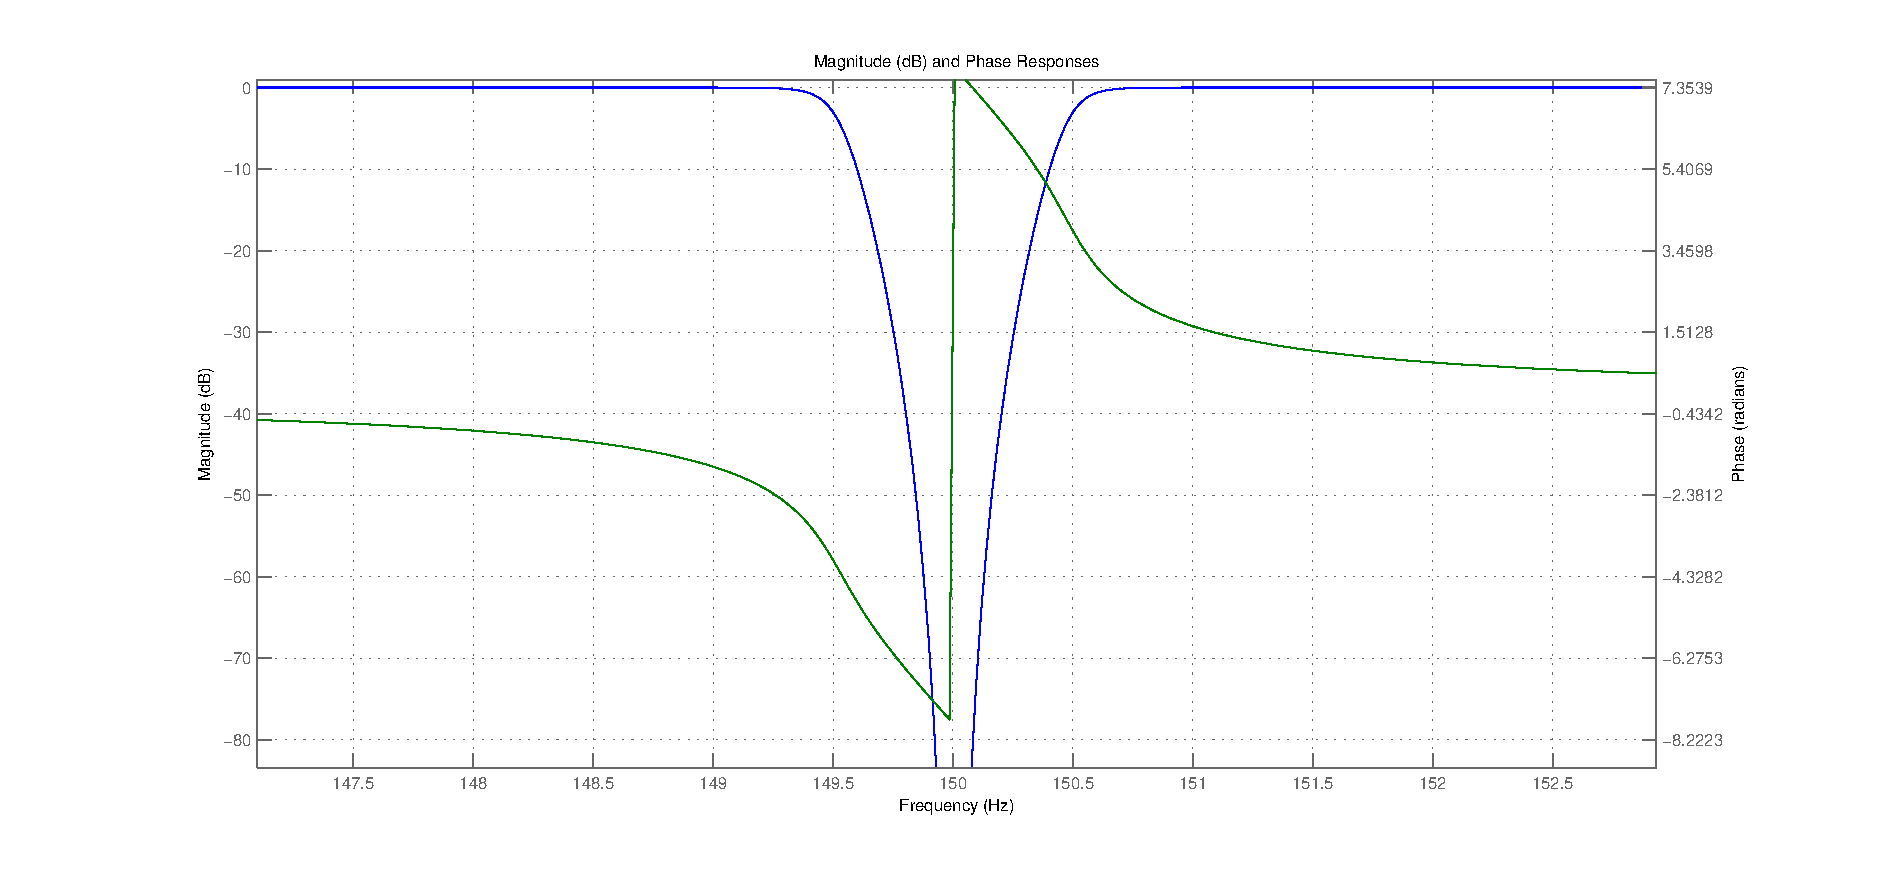
\includegraphics[width=\textwidth]{ECG_BASELINE/figures/3rd_harm_360.eps}
\caption{Charakterystyka amplitudowa i fazowa filtru Butterwortha do usuwania 3. harmonicznej szumu sieciowego 50 Hz dla $f_s=360 Hz$}
\label{fig:3rd_360}
\end{figure}

\subsection{Średnia krocząca}

Średnia krocząca (MA -- \emph{Moving Average}) jest jednym z najprostszych filtrów cyfrowych. Równanie średniej kroczącej jest następujące

\begin{equation}
y[i] = \frac{1}{M}\sum_{j=0}^{M-1}x[i - j]
\end{equation}

gdzie $y$ jest sygnałem wyjściowym, $x$ -- sygnałem wejściowym, zaś $M$ to ilość próbek wchodzących w skład średniej. 

Średnia krocząca jest filtrem o działaniu uśredniającym, o właściwościach dolnoprzepustowego filtru o skończonej odpowiedzi impulsowej. W celu zastosowania tego filtru do usunięcia falowania izolinii, konieczne jest odjęcie otrzymanego wyjścia filtru od każdej próbki sygnału wejściowego, zgodnie z równaniem

\begin{equation}
y_{hp}[i] = x[i] - y[i]
\end{equation}

Implementacja średniej kroczącej zawarta w module ECG\_BASELINE zmodyfikowana została w sposób umożliwiający jej wywołanie z podaniem czasu uśredniania $t_a$ oraz częstotliwości próbkowania sygnału $f_s$. Ilość próbek wchodzących w skład średniej $M$ jest wtedy wyliczana z wzoru

\begin{equation}
M = \ceil{t_a \cdot f_s}
\end{equation}


\subsection{Rozszerzony Filtr Kalmana}
Konstrukcja filtru Kalmana powstała w oparciu o \cite{Sameni2005-1, Sameni2005-2} i przedstawiona w formie algorytmicznej. Podstawy teoretyczne metody oraz szczegóły poszczególnych kroków algorytmu znajdują się w dalszej części rozdziału.

Algorytm odszumiania zapisu EKG przy użyciu rozszerzonego filtru Kalmana
\begin{enumerate}
\item Usuń izolinię sygnału EKG (np. przy użyciu średniej kroczącej)
\item Zidentyfikuj parametry modelu nieliniowego
\item Dopasuj model do średniego przebiegu wejściowego sygnału
\item Przeprowadź filtrację sygnału, wykorzystując rozszerzony, wygładzający filtr Kalmana
\end{enumerate}

Dyskretny Filtr Kalmana estymuje stan dyskretnego systemu dynamicznego, opisanego liniowym, stochastycznym równaniem różnicowym:
\begin{equation}
 x_k = Ax_{k-1} + Bu_{k-1} + w_{k-1}
\end{equation}
z wyjściem opisanym równaniem:
\begin{equation}
 z_k = Hx_k + \upsilon_k
\end{equation}

Zmienne losowe $w_k, \upsilon_k$ reprezentują odpowiednio szum procesu i pomiaru. Zakładamy, że są one niezależne od siebie i charakteryzują się rozkładem normalnym:
\begin{equation}
\begin{split}
 p(w) \backsim N(0,Q) \\
 p(\upsilon) \backsim N(0,R)
 \end{split}
\end{equation}

\begin{figure}
\centering
	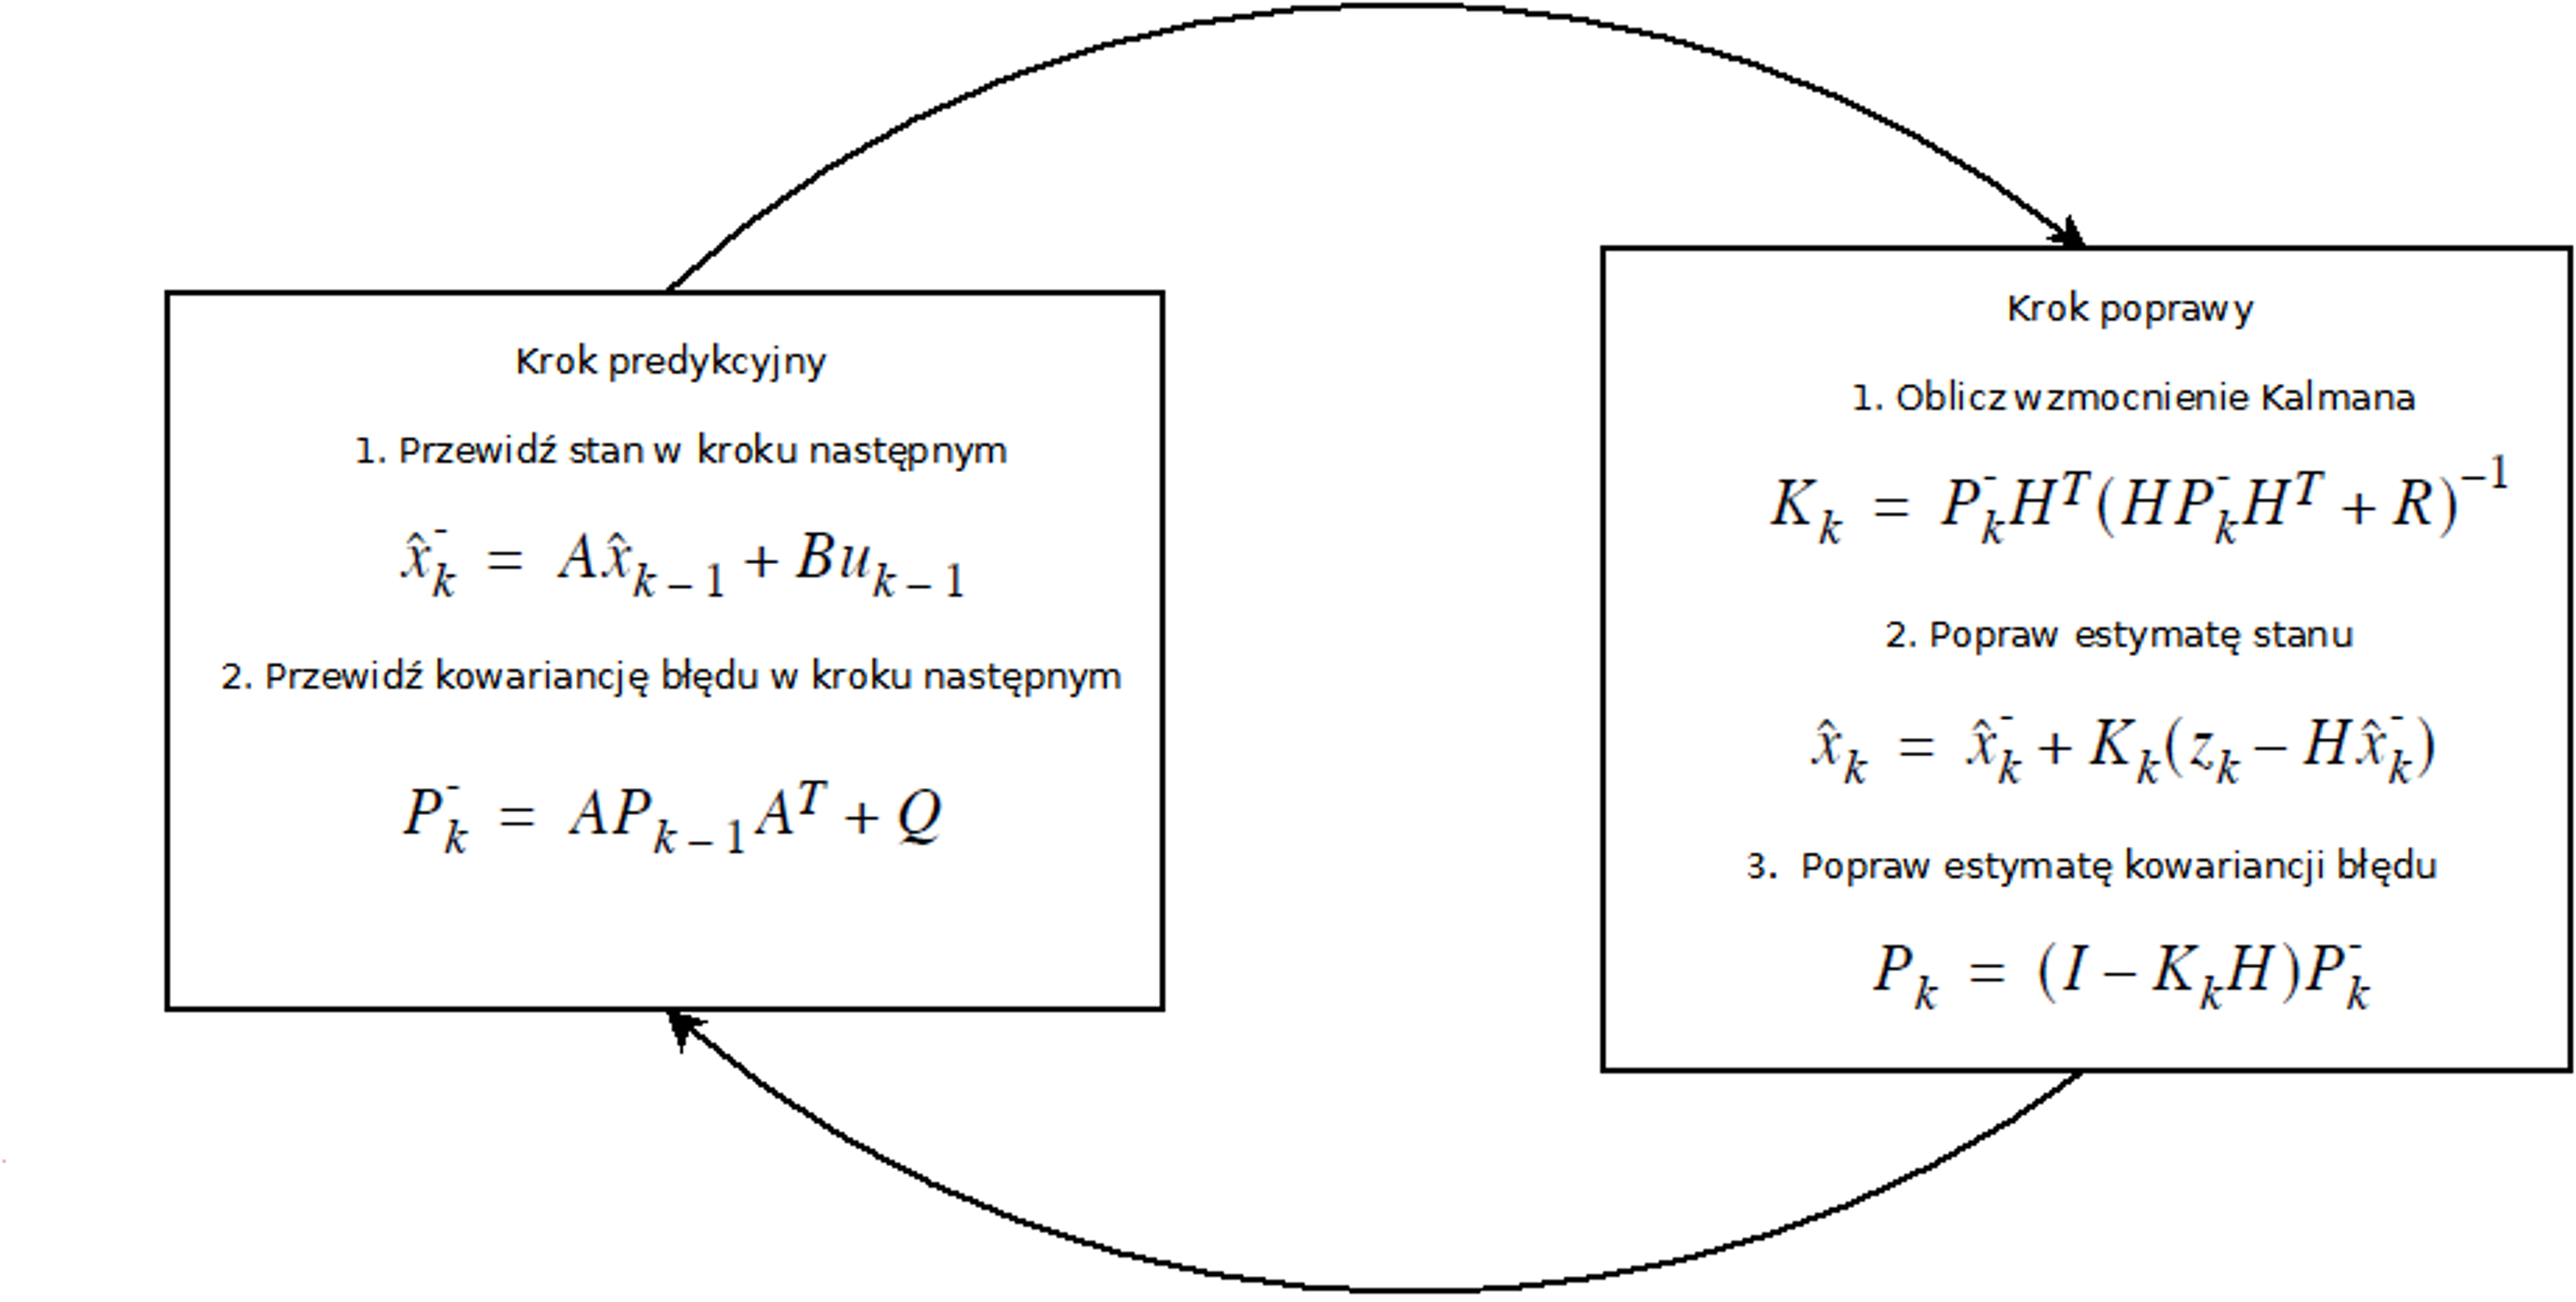
\includegraphics[width=\textwidth]{ECG_BASELINE/figures/KF.png}
\caption{Działanie filtru Kalmana}
\label{Kalman}
\end{figure}

Rysunek \ref{Kalman} przedstawia schemat ideowy dyskretnego filtru Kalmana. W pierwszym kroku („predykcyjnym”) estymowany jest obecny stan modelu na podstawie stanu poprzedniego. Następnie, krok „korekcyjny” służy uwzględnieniu obecnych pomiarów i naniesieniu poprawki na stan. Wpływ stanu poprzedniego i obecnego pomiaru na stan obecny jest determinowany przez macierze $R$ i $Q$, wyznaczane w procesie identyfikacyjnym. Występująca w równaniach macierz $P$ oznacza kowariancję estymaty błędu modelu. Rozszerzony filtr Kalmana, w przeciwieństwie do swej klasycznej wersji, estymuje stan nieliniowego systemu dynamicznego, linearyzując go w otoczeniu stanu poprzedniego, zakładając, że chwilowe wartości $w_k, \upsilon_k$ wynoszą 0. 
Wygładzający filtr Kalmana dokonuje estymacji stanu, wykorzystując wszystkie pomiary sygnału, pobrane w stałych odstępach czasu. Wykorzystano tu fakt, że filtracji sygnału dokonujemy off-line, a zatem wszystkie pomiary zostały już zgromadzone. W tym celu najczęściej wykorzystuje się algorytm Rachua-Tunga-Striebela, który dzieli się na dwa etapy. W pierwszym kroku uruchamia się zwyczajny filtr Kalmana i zachowuje się estymaty stanu $x_{k|k}$ i kowariancje $P_{k|k}$ do użycia w kroku drugim. Następny etap polega na obliczeniu wygładzonych estymat stanu $x_{k|n}$ i kowariancji $P_{k|n}$, zaczynając od końca sygnału, z wykorzystaniem następujących, rekurencyjnych równań:
\begin{equation}
\begin{cases}
	\hat{x}_{k|n} &= \hat{x}_{k|k} + C_k(\hat{x}_{k+1|n} - \hat{x}_{k+1|k}) \\
	P_{k|n} &= P_{k|k} + C_k(P_{k+1|n} - P_{k+1|k})C_{k}^T
\end{cases}
\end{equation}
Gdzie:
\begin{equation}
\begin{split}
	C_k = P_{k|k} \cdot A_{k}^T \cdot P_{k+1|k} ^{-1}
\end{split}
\end{equation}

\subsubsection{Model matematyczny}
W oparciu o \cite{Sameni2005-1}, przyjęty następujący, dyskretny model matematyczny, opisany we współrzędnych biegunowych:
\begin{equation}
\begin{cases}
	\theta[k+1] &= \theta[k] + \omega \Delta \\
	z[k+1] &= \sum_{i \in {P, Q, R, S, T} } \Delta a_i \Delta \theta_i \exp \left({- \frac{\Delta \theta_i^2}{2 b_i^2}} \right) + z[k] + N \Delta
\end{cases}
\label{eq:model1}
\end{equation}

Zmiennymi stanu modelu są: $\theta$ -- faza sygnału i $z$ -- jego amplituda. Ponadto, $\Delta$ to czas próbkowania, a $\Delta \theta_i = (\theta - \theta_i)mod(2 \pi)$. $N$ to addytywny szum, modelujący izolinię oraz inne zakłócenia procesowe. Rzut powyższego modelu na oś $z$ przedstawia sygnał EKG.

W celu wykorzystania powyższego modelu w implementacji rozszerzonego filtru Kalmana, należy również uzyskać jego zlinearyzowaną postać. Przyjmując:
\begin{equation}
\begin{cases}
	\theta[k+1] &= F(\theta, z, \omega, k) \\
	z[k+1] &=  G(\theta, z, a_i, \theta_i, b_i, N, k)
\end{cases}
\label{eq:model-lin1}
\end{equation}

następujące równania przedstawiają zlinearyzowany model ze względu na zmienne stanu $\theta$ i $z$. 

\begin{equation}
\begin{split}
	\frac{\partial F}{\partial z} &= 0 \\
	\frac{\partial F}{\partial \theta} &= \frac{\partial G}{\partial z} = 1 \\
	\frac{\partial G}{\partial \theta} &= \sum_{i \in {P, Q, R, S, T} } - \Delta a_i \left( 1 - \frac{\Delta \theta_i^2}{b_i^2} \right) \exp \left({- \frac{\Delta \theta_i^2}{2 b_i^2}} \right)
\end{split}
\label{eq:model-lin2}
\end{equation}

Podobnie, układ równań~\ref{eq:model-lin3} to wynik linearyzacji równania~\ref{eq:model-lin1} w zależności od szumów procesowych.

\begin{equation}
\begin{split}
	\frac{\partial F}{\partial a_i} &= \frac{\partial F}{\partial b_i} = \frac{\partial F}{\partial \theta_i} = \frac{\partial F}{\partial N} = 0 \\
	\frac{\partial F}{\partial \omega} &= \Delta \\
	\frac{\partial G}{\partial a_i} &= - \Delta \cdot \Delta \theta_i \exp \left({- \frac{\Delta \theta_i^2}{2 b_i^2}} \right), i \in {P, Q, R, S, T} \\
	\frac{\partial G}{\partial b_i} &= - \Delta a_i \frac{\Delta \theta_i^3}{b_i^3} \exp \left({- \frac{\Delta \theta_i^2}{2 b_i^2}} \right) \\
	\frac{\partial G}{\partial \omega} &= 0 \\
	\frac{\partial G}{\partial \theta_i} &= \Delta a_i \left[1 - \frac{\Delta \theta_i^2}{b_i^2} \right] \exp \left({- \frac{\Delta \theta_i^2}{2 b_i^2}} \right) \\
	\frac{\partial G}{\partial N} &= \Delta 
\end{split}
\label{eq:model-lin3}
\end{equation}

Szum procesowy może być oznaczony jako $\underline{w}_k = \left[ a_P,...,a_T,b_P,...,b_T, \theta_P,...,\theta_T,\omega,N \right]$, a $Q_k = E \{\underline{w}_k, \underline{w}_k^T \}$. Tym samym model dynamiczny jest przygotowany do wykorzystania w rozszerzonym filtrze Kalmana.

\section{Testy filtrów}

\subsection{Filtr Butterwortha}

Wyniki części przeprowadzonych testów nowych zestawów współczynników dla fitru Butterwortha przedstawiono na rysunkach~\ref{fig:bw_removal_comparison},~\ref{fig:bw_removal_zoom},~\ref{fig:50hz_comparison},~\ref{fig:50hz_zoom}.

\begin{figure}[H]
\centering
	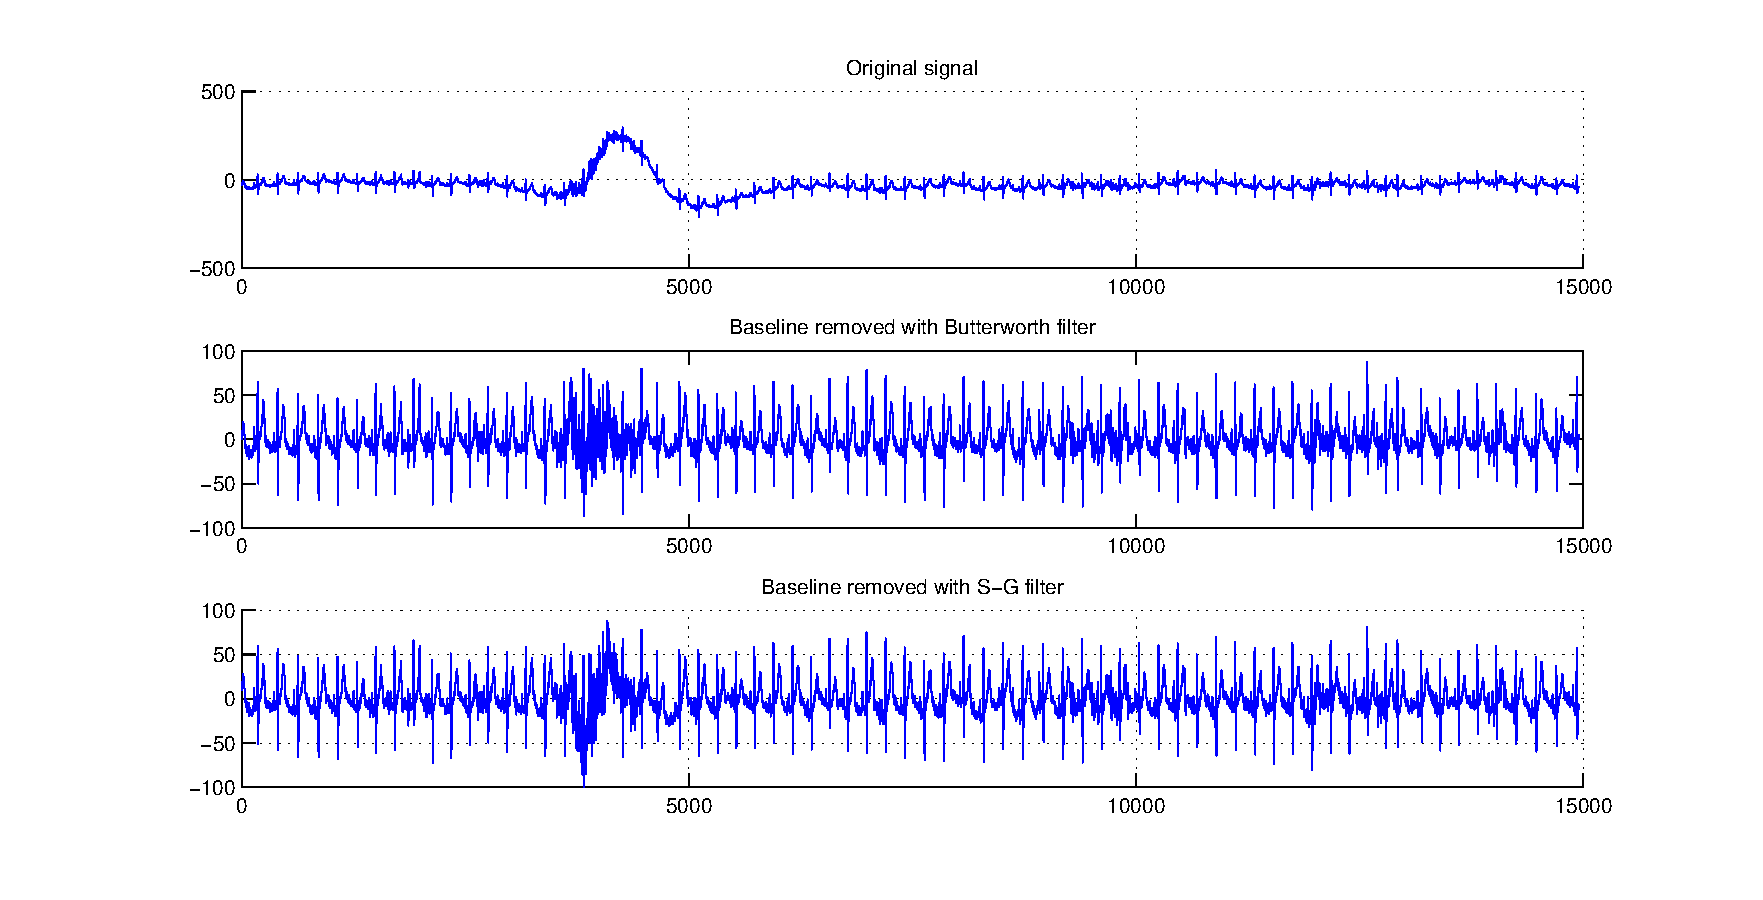
\includegraphics[width=\textwidth]{ECG_BASELINE/figures/250_baseline_comparison.eps}
\caption{Porównanie działania filtru Butterwortha i filtru Savitzky'ego-Golay'a do usuwania falowania izolinii z sygnału próbkowanego z częstotliwością $f_s=250 Hz$}
\label{fig:bw_removal_comparison}
\end{figure}

\begin{figure}[H]
\centering
	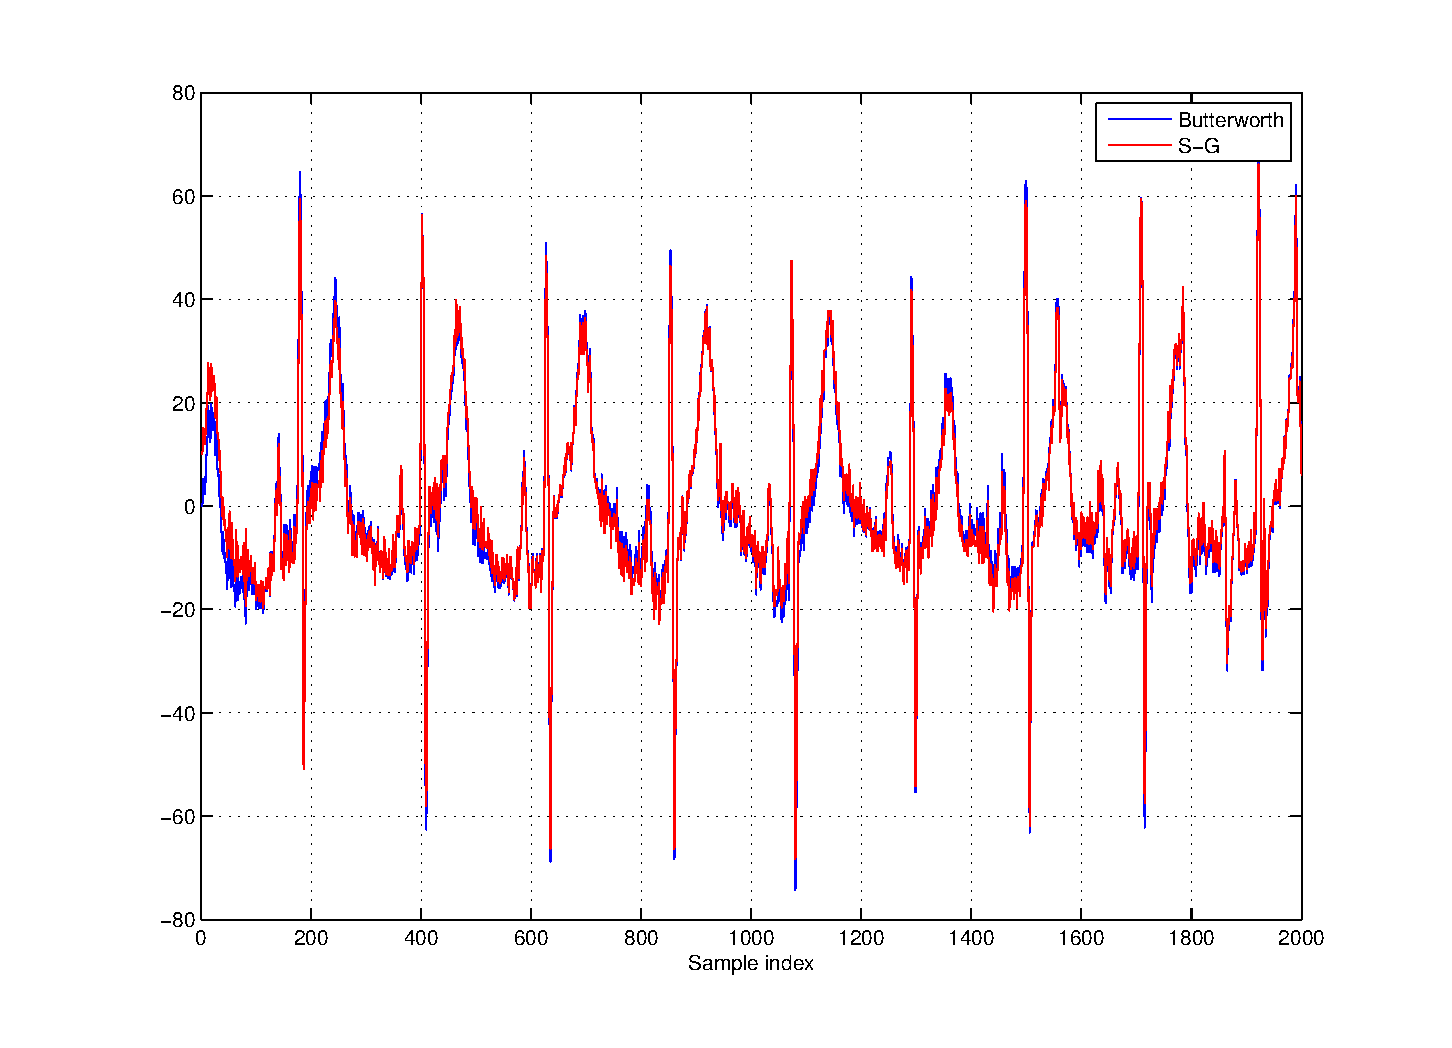
\includegraphics[width=0.7\textwidth]{ECG_BASELINE/figures/zoom_butter_sg.eps}
\caption{Powiększony fragment przebiegów wyjścia filtru S-G i Butterwortha.}
\label{fig:bw_removal_zoom}
\end{figure}

\begin{figure}[H]
\centering
	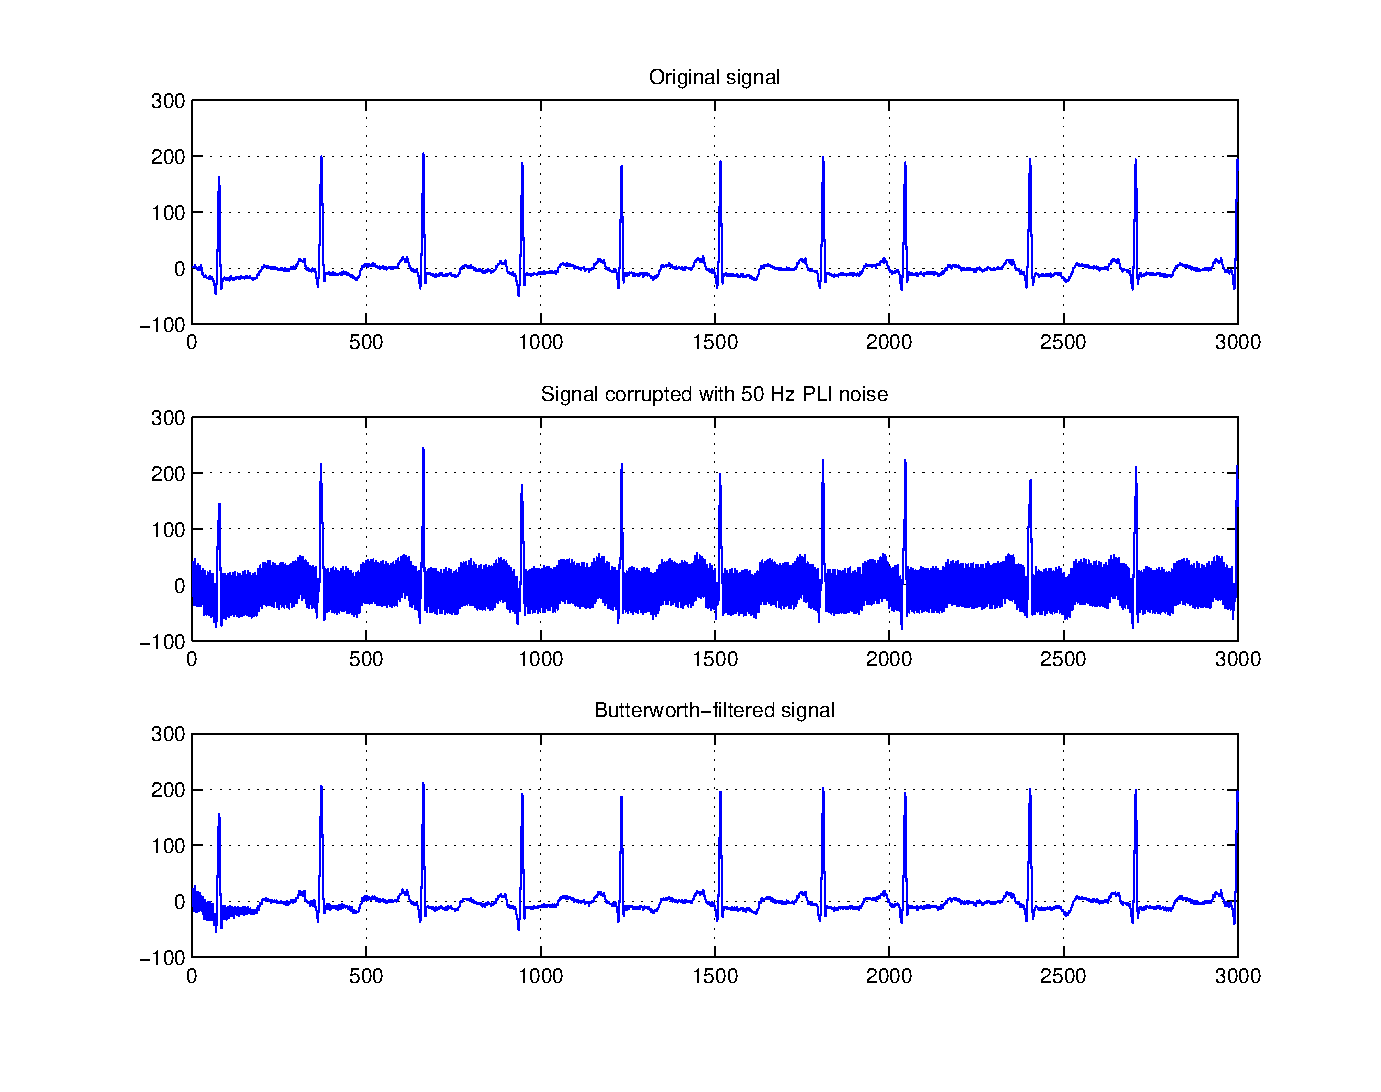
\includegraphics[width=1.05\textwidth]{ECG_BASELINE/figures/50hz.eps}
\caption{Zestawienie sygnałów: przed zaszumieniem, sygnału zaszumionego oraz wyjścia filtru Butterwortha dla szumu sieciowego 50 Hz}
\label{fig:50hz_comparison}
\end{figure}

\begin{figure}[H]
\centering
	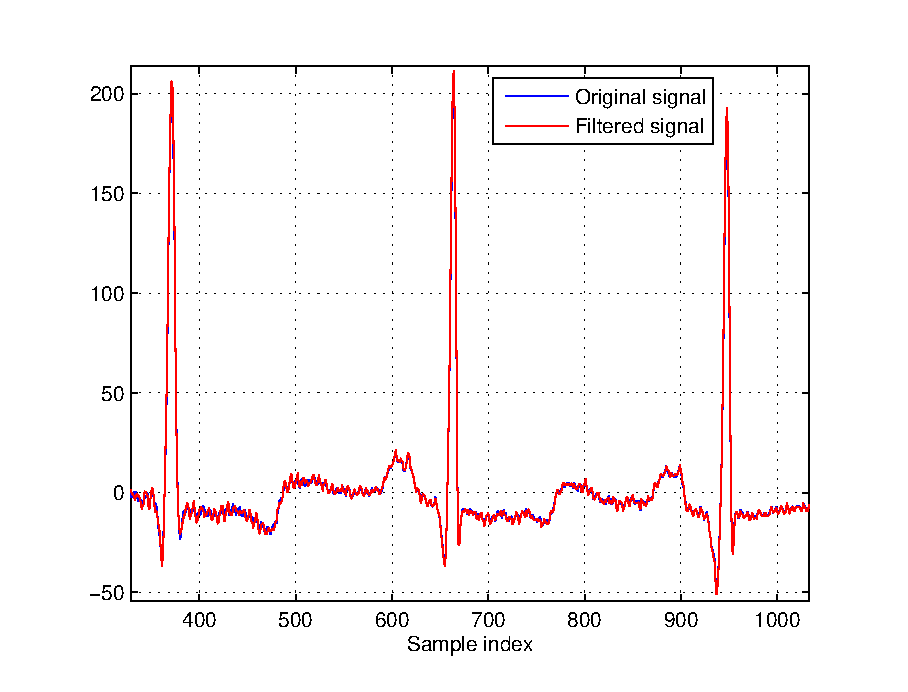
\includegraphics[width=\textwidth]{ECG_BASELINE/figures/50hz_zoom.eps}
\caption{Porównanie wyników filtracji Butterwortha do usuwania szumu sieciowego 50 Hz z sygnałem przed zaszumieniem}
\label{fig:50hz_zoom}
\end{figure}


\subsubsection{Filtr Kalmana}
Rysunek ~\ref{fig:KalmanOutput} przedstawia przykładowy efekt działania rozszerzonego filtru Kalmana, zaś ~\ref{fig:KalmanSNR} - zależność między stosunkiem sygnału użytecznego danych wejściowych i wyjściowych metody. W celu uzyskania mierzalnych wyników, do sygnału wejściowego z usuniętą izolinią dodawano szum biały o zadanej mocy. Zaobserwowano znaczną poprawę sygnału po przeprowadzeniu filtracji, co ma swój wymiar zarówno jakościowy, jak i ilościowy. 

\begin{figure}[H]
\centering
	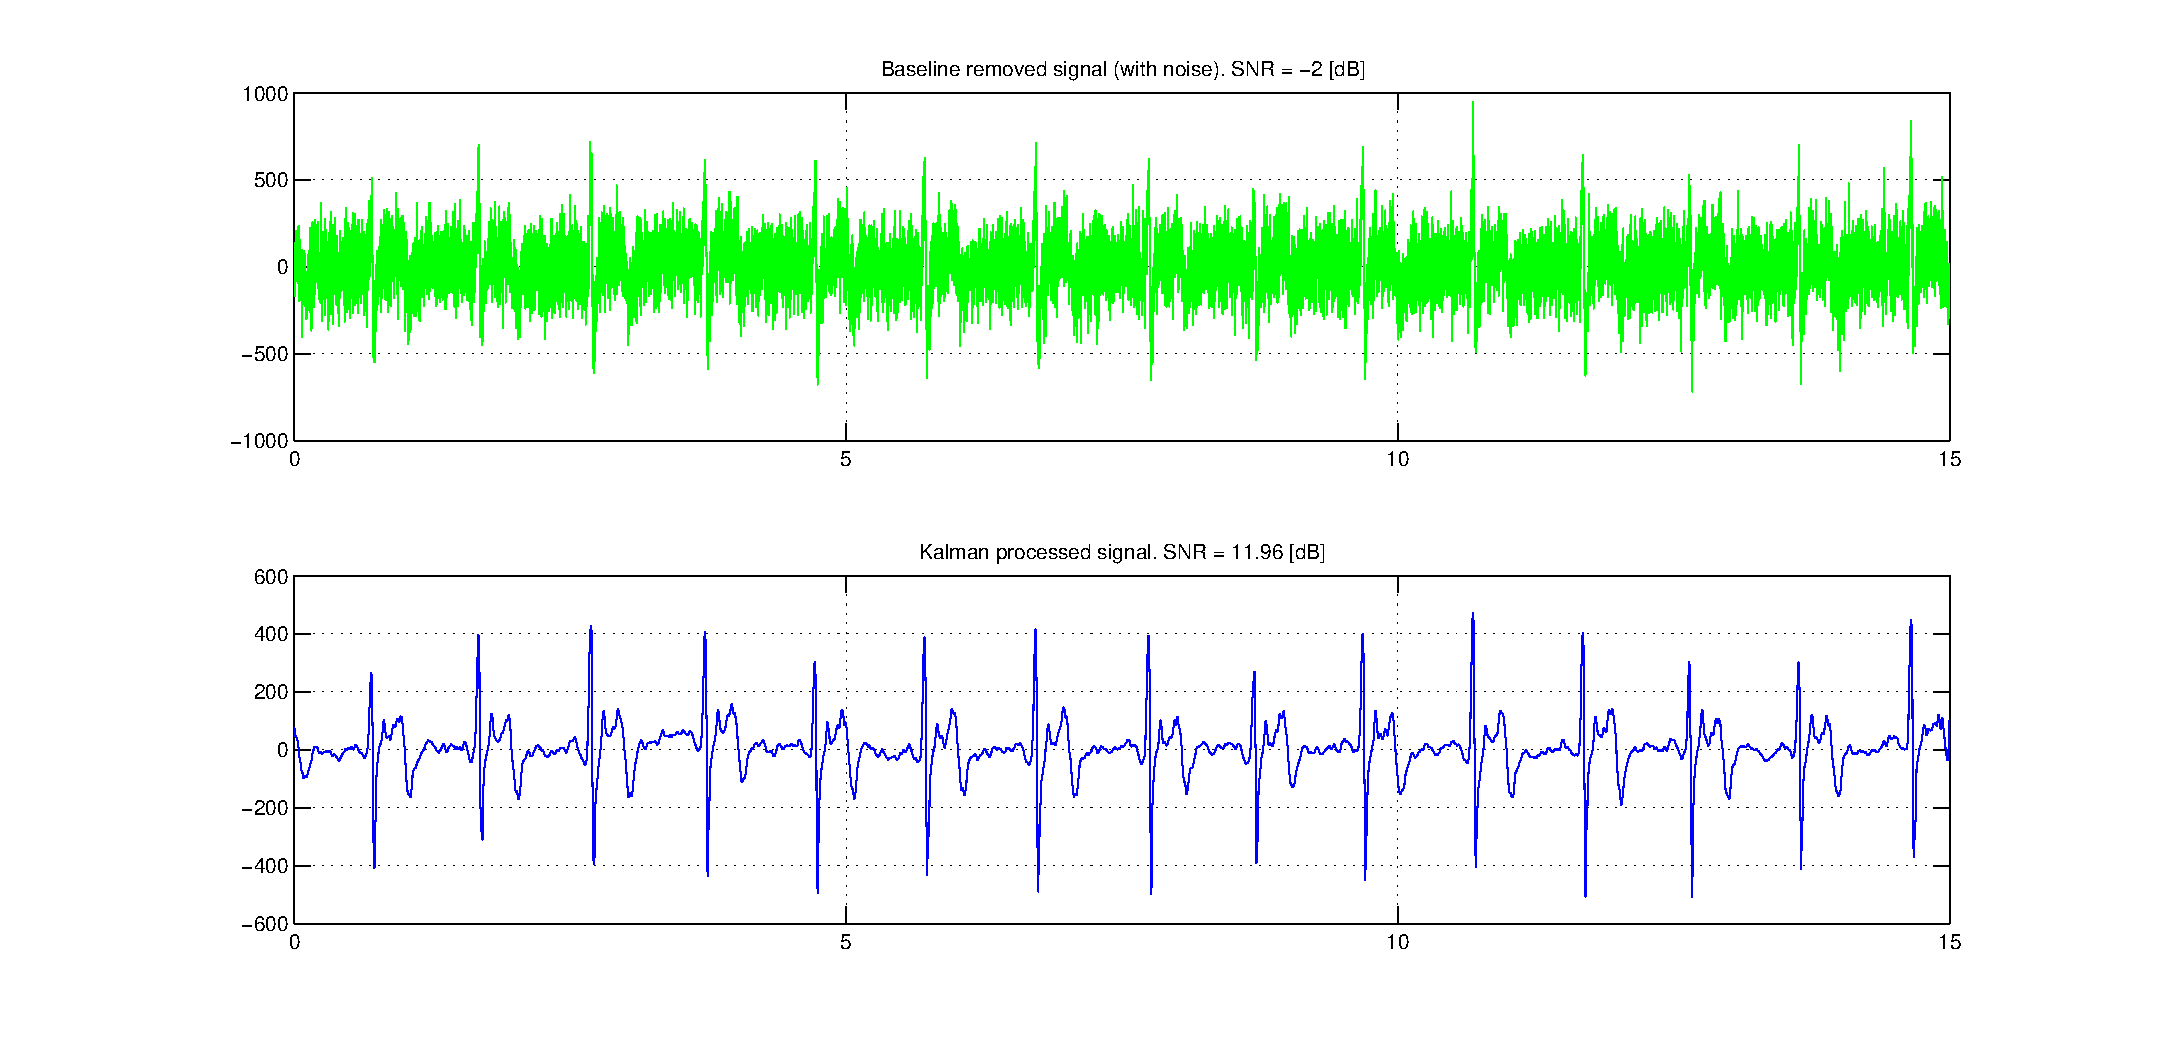
\includegraphics[width=\textwidth]{ECG_BASELINE/figures/hardCoreNoise.eps}
\caption{Wynik filtracji sygnału EKG za pomocą rozszerzonego filtru Kalmana}
\label{fig:KalmanOutput}
\end{figure}

\begin{figure}[H]
\centering
	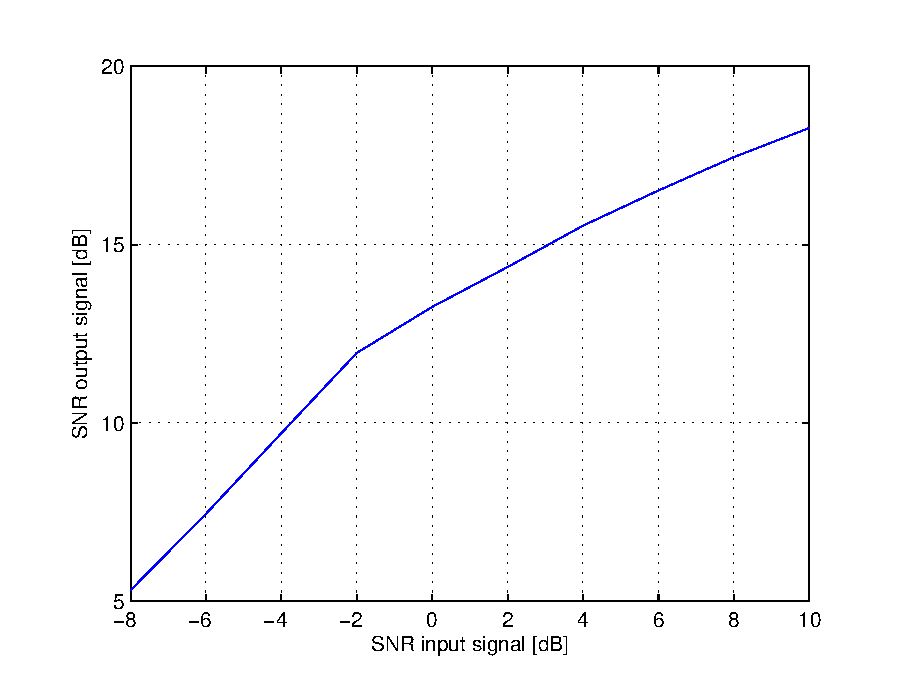
\includegraphics[width=0.9\textwidth]{ECG_BASELINE/figures/snrInOut.eps}
\caption{Zależność między SNR sygnału wejściowego i wyjściowego filtru Kalmana}
\label{fig:KalmanSNR}
\end{figure}



\subsection{Opis implementacji}
Moduł obliczeniowy ECG\_BASELINE zaimplementowany jest w języku C++. Poprawność jego działania testowana była przy użyciu dwóch kompilatorów: Microsoft Visual Studio 2012 oraz gcc w wersji 4.6 (zarówno w wersji MinGW, jak i przeznaczonej dla systemów GNU/Linux).

W module wykorzystane zostały dwie biblioteki zewnętrzne:

\begin{itemize}
\item Eigen -- biblioteka szablonowa C++ zawierająca implementacje operacji macierzowych
\item ALGLIB -- biblioteka C++ zawierająca implementacje wielu algorytmów numerycznych, transformat itp. 
\end{itemize}

Z biblioteki ALGLIB do określenia parametrów modelu syntetycznego sygnału EKG użyta została metoda Levenberga-Marquardta, zaimplementowana w funkcji \texttt{lsfitfit()} z pliku nagłówkowego \texttt{interpolation.h}. 

Średnia krocząca, filtr Butterwortha i filtr Savitzky'ego-Golay'a zaimplementowane zostały funkcje bezstanowe, jednak w porównaniu do poprzedniej wersji, refaktoryzacji uległ interfejs filtru Butterwortha. Do przechowywania współczynników tego filtru utworzona została nowa klasa, przedstawiona w uproszczony sposób na diagramie~\ref{fig:ButterCoefficients_uml}. Wszystkie pola klasy inicjalizowane są w konstruktorze.

\begin{figure}[H]
\centering
	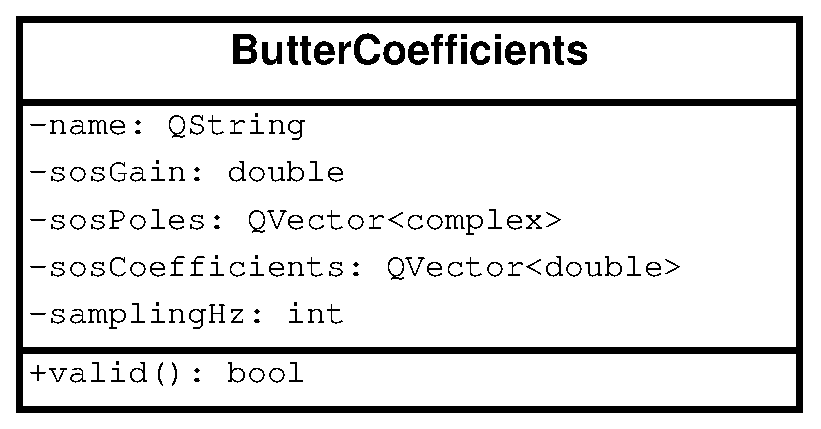
\includegraphics[width=0.4\textwidth]{ECG_BASELINE/figures/ButterCoefficients.eps}
\caption{Diagram UML klasy \textit{ButterCoefficients}}
\label{fig:ButterCoefficients_uml}
\end{figure}

Taka zmiana pozwala na wygodną obsługę wielu zestawów współczynników, a przy użyciu odpowiedniego GUI -- również ich wprowadzanie przez użytkownika. Predefiniowane zestawy współczynników pobiera się przy użyciu funkcji o prototypie \texttt{const QVector<ButterCoefficients>\& predefinedButterCoefficientSets()} zadeklarowanej w pliku nagłówkowym \texttt{butter.h}.

Implementacja filtru Kalmana również udostępnia prosty w użyciu interfejs. Stworzona klasa \textit{KalmanFilter} udostępnia tylko jedną metodę publiczną, zwracającą przefiltrowany sygnał dla surowego wejścia. Metody prywatne odzwierciedlają przedstawiony wyżej algorytm, w razie potrzeby dzielono je na mniejsze części. Powstało w sumie kilkadziesiąt funkcji prywatnych, starano się bowiem, by były one możliwie krótkie i pisane na tym samym poziomie abstrakcji. Metody wykonujące podstawowe operacje na zbiorach danych umieszczono w statycznej klasie \textit{BaseLineUtils}. Poniżej przedstawiono diagram UML klasy \textit{KalmanFilter}, z wyróżnieniem metody publicznej i kilku najważniejszych metod prywatnych. Przedstawione na diagramie atrybuty klasy są ustawiane w jej konstruktorze. Dla filtru Kalmana również utworzono funkcję bezstanową, umożliwiającą filtrowanie podanego wektora próbek.

Podsumowując, dostęp do zaimplementowanych w module metod filtrujących odbywa się poprzez wykorzystanie następujących funkcji bezstanowych, zadeklarowanych w odpowiednich plikach nagłówkowych:

\begin{itemize}

\item \texttt{QVector<double> processMovAvg(const QVector<double> \&signal, int samplingFrequencyHz, double averagingTimeS);}\\ lub \\ \texttt{QVector<double> processMovAvg(const QVector<double>\& signal, int windowSize);}
\item \texttt{QVector<double> processButter(const QVector<double>\& signal, const ButterCoefficients \&coefficients);}
\item \texttt{QVector<double> processSGolay(const QVector<double>\& ecgData, const int deg = 3, const int frame = 500, QVector<double>* baselineModel = 0);}
\item \texttt{QVector<double> processKalman(const QVector<double>\& input, double samplingFrequency);}
\end{itemize}

\begin{figure}[H]
\centering
	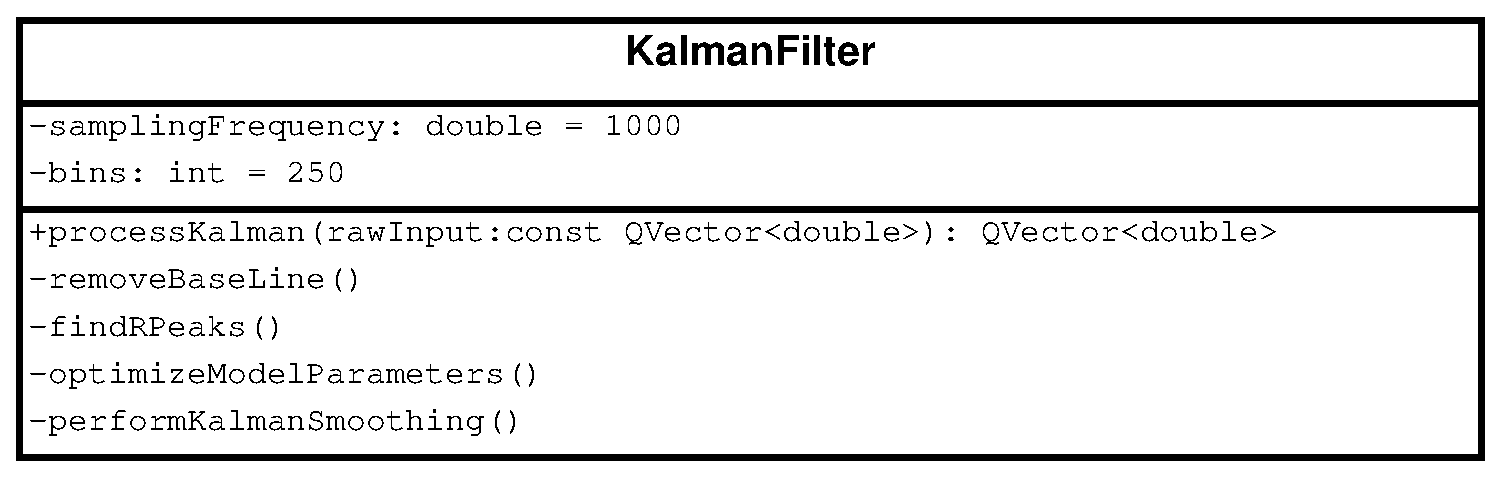
\includegraphics[width=0.7\textwidth]{ECG_BASELINE/figures/KalmanFilter.eps}
\caption{Diagram UML klasy \textit{KalmanFilter}}
\label{KF-UML}
\end{figure}


\subsubsection{Diagramy sekwencji UML}

\begin{figure}[H]
\centering
	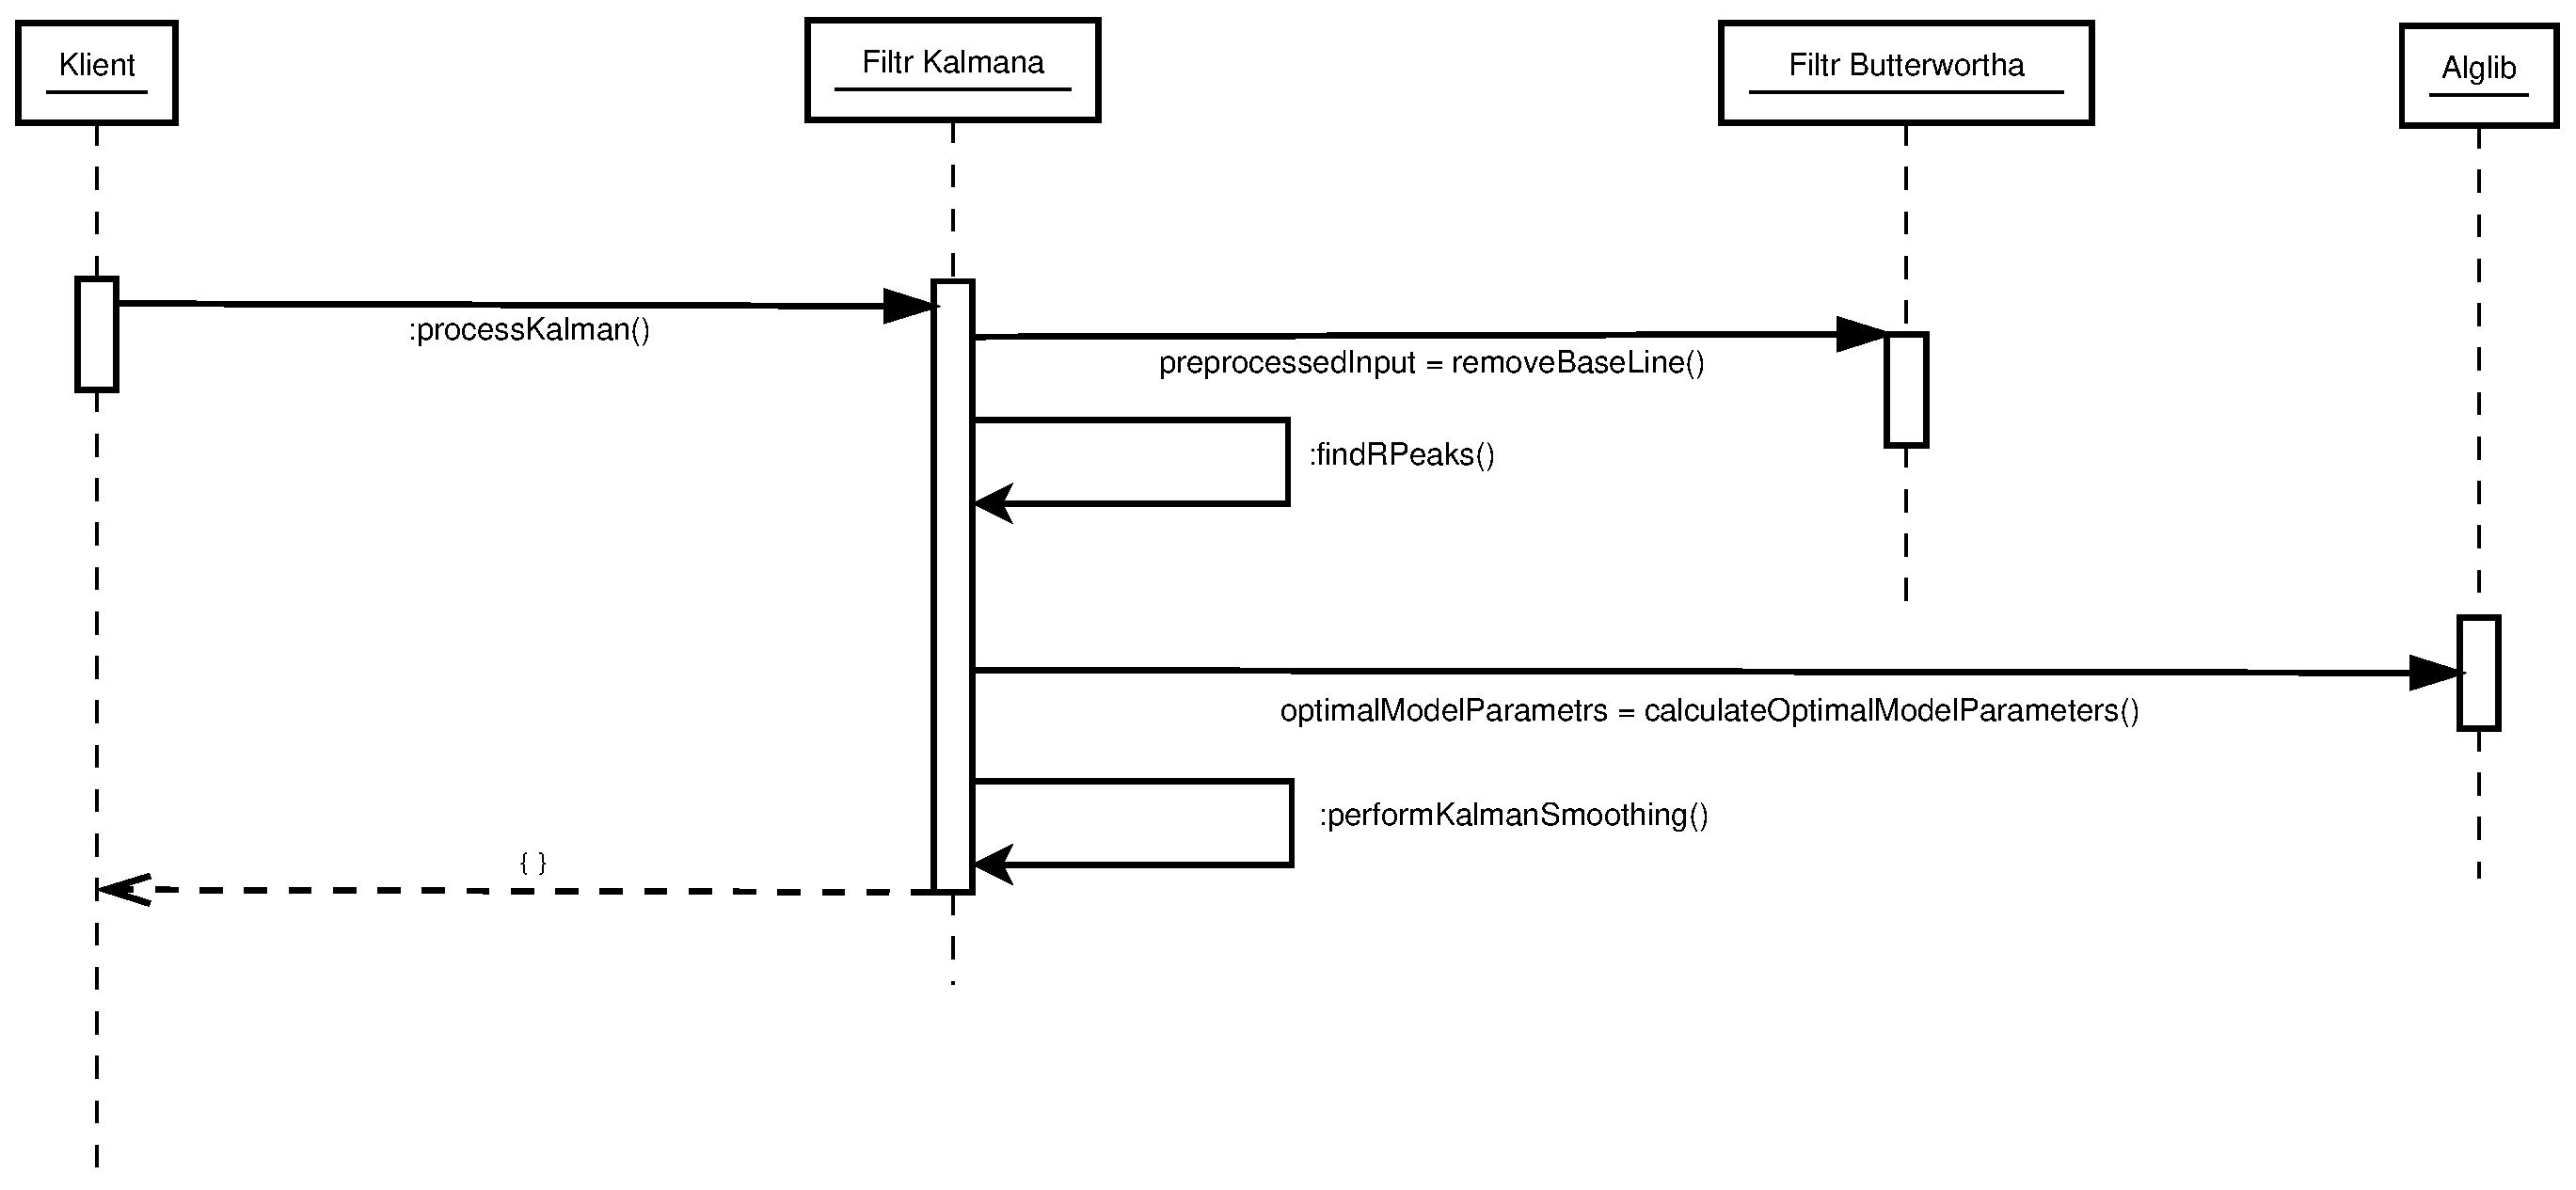
\includegraphics[width=\textwidth]{ECG_BASELINE/figures/KalmanDiagram.eps}
\caption{Diagram sekwencji klasy \textit{KalmanFilter}}
\label{KF-Diagram}
\end{figure}

\begin{figure}[H]
\centering
	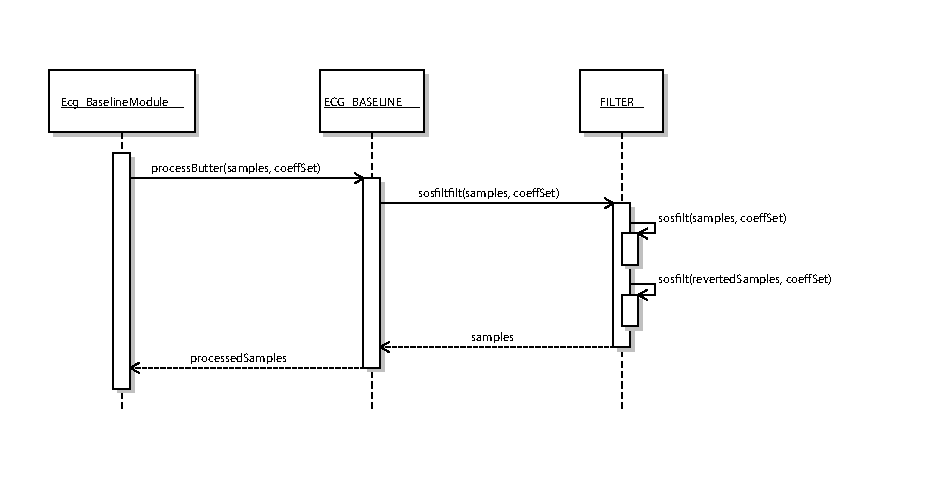
\includegraphics[width=1.1\textwidth]{ECG_BASELINE/figures/butter_seq.pdf}
\caption{Diagram sekwencji dla przypadku użycia filtru Butterwortha.}
\label{MA-seq}
\end{figure}

\begin{figure}[H]
\centering
	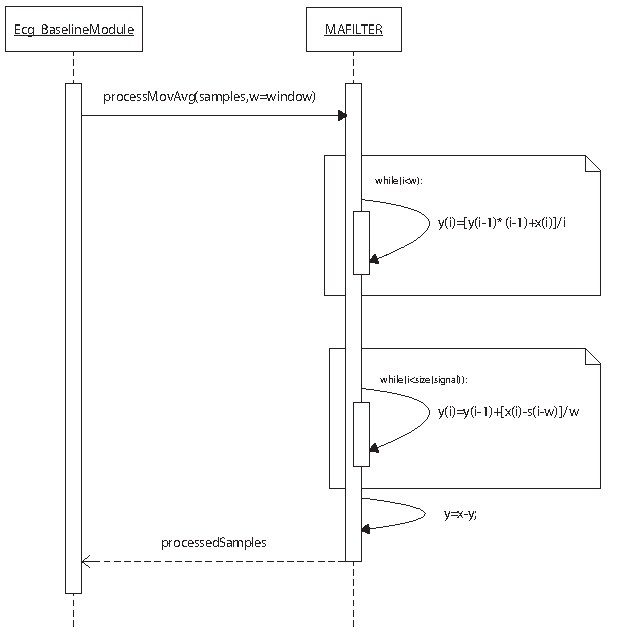
\includegraphics[width=0.8\textwidth]{ECG_BASELINE/figures/ma_seq.pdf}
\caption{Diagram sekwencji dla przypadku użycia średniej kroczącej. Źródło: \cite{Baseline2013}}
\label{MA-seq}
\end{figure}

\begin{figure}[H]
\centering
	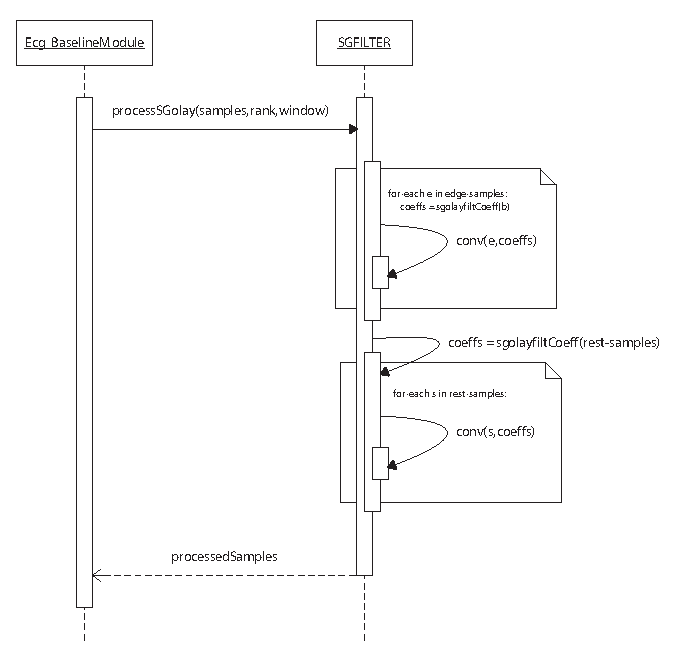
\includegraphics[width=0.8\textwidth]{ECG_BASELINE/figures/sg_seq.pdf}
\caption{Diagram sekwencji dla przypadku użycia filtru Savitzky'ego-Golay'a. Źródło: \cite{Baseline2013}}
\label{MA-seq}
\end{figure}




\subsection{Podsumowanie}
W ramach projektu z powodzeniem zaimplementowano rozszerzony filtr Kalmana dla sygnału EKG, wprowadzono zmiany w interfejsie średniej kroczącej oraz zrefaktoryzowano i dodano nowe zestawy współczynników do filtru Butterwortha. Nowe zestawy współczynników pozwalają na usunięcie z sygnału EKG falowania izolinii oraz szumu sieciowego (50 Hz). 

W przypadku zakłócenia o wielu składowych częstotliwościowych i rozkładzie zbliżonym do normalnego, najlepsze wyniki daje zastosowanie rozszerzonego filtru Kalmana. Jest on znacznie bardziej złożony od typowych filtrów FIR i IIR (jego implementacja w języku C++ wymaga około tysiąca linii kodu) i wymaga znacznie dłuższych obliczeń -- dla zapisu trwającego 30 minut ($f_s = 360 Hz$), czas filtracji wynosi około 45 sekund na komputerze z procesorem klasy Intel i5.

Podsumowując -- usuwanie rzeczywistych zakłóceń w sygnale EKG jest trudne, głównie ze względu na niewielką amplitudę sygnału oraz jego pasmo -- w dużej mierze pokrywające się z pasmem szumów. Problem usunięcia falowania linii izoelektrycznej jest szeroko opisywany w literaturze, zaś zaimplementowane w module ECG\_BASELINE rozwiązania uznać można za spełniające wymagania. Zakłócenia pochodzenia sieciowego (PLI -- \emph{Power Line Interference}) są również niemal całkowicie usuwalne przy użyciu pasmowozaporowych filtrów Butterwortha z odpowiednimi zestawami współczynników. 
